\chapter*{Installation}
\label{chap:installation}
\begin{figure}[H]
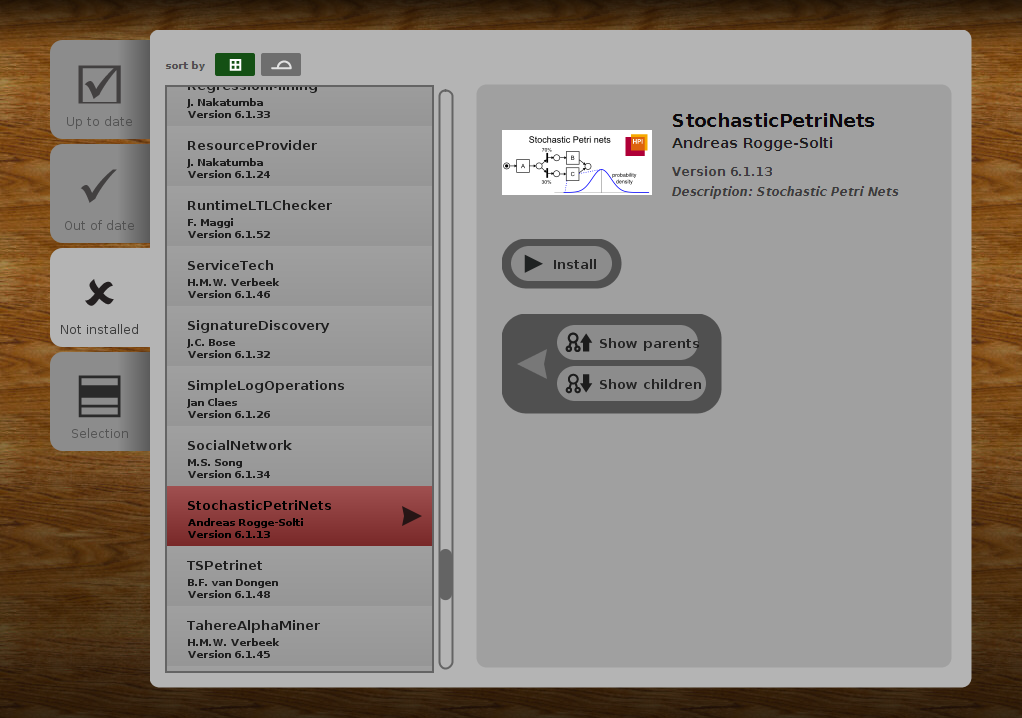
\includegraphics[width=\textwidth]{installer.png}
\caption{Select \& install the StochasticPetriNet Package.}
\label{fig:installation}
\end{figure}


\subsubsection*{About}
The StochasticPetriNet package contains plugins to import and export stochastic Petri nets in the Petri net markup \texttt{.pnml} format.
It allows to convert aligned Logs / Petri net models, i.e., Manifests (output of the \emph{PNetReplayer}-plugin), to stochastic Petri nets.
A visualizer is included. And a prediction experiment comparing predicted times from Transition system based prediction and Petri net based predictions of remaining process durations.

\pagebreak
\section*{Optional: Install R for log spline density estimations}
\label{sec:optional} 
If you want to try the Log-spline density estimator, you need to install the R-project. \url{http://www.r-project.org/}
It is based on the CRAN \texttt{logspline} package by Charles Koopenberg \url{http://cran.r-project.org/web/packages/logspline/index.html}

Proceed with the following steps:
\begin{itemize}
  \item Download and install R \url{http://www.r-project.org/}
  \item startup R and run \texttt{ install.packages("logspline")}
  \item install the binaries for the Java-to-R bridge \texttt{ install.packages("rJava")}
  \item the \mypackagename package needs to point java to the native JRI library, that was installed with rJava. Make sure to add the VM-argument:\\
  -Djava.library.path=\ldots~ points to that binary. 
  \item make sure your environment variable \texttt{R\_HOME} points to your R installation containing the binaries (for linux, this might be \texttt{/usr/lib/R}, or \texttt{/usr/lib64/R})
\end{itemize}

\subsubsection{Note:}
The license of the plug-in will be \textbf{GPL}, if you use it with R and the logspline package.
